\documentclass{beamer}
\usepackage[latin1]{inputenc}

\usetheme{Madrid}
\usecolortheme{default}
\usepackage{amsmath}
\usepackage{amssymb,amsfonts,amsthm}
\usepackage{txfonts}
\usepackage{tkz-euclide}
\usepackage{listings}
\usepackage{adjustbox}
\usepackage{array}
\usepackage{tabularx}
\usepackage{gvv}
\usepackage{lmodern}
\usepackage{circuitikz}
\usepackage{tikz}
\usepackage{graphicx}
\usepackage{gensymb}
\usepackage{physics}

\setbeamertemplate{page number in head/foot}[totalframenumber]

\usepackage{tcolorbox}
\tcbuselibrary{minted,breakable,xparse,skins}



\definecolor{bg}{gray}{0.95}
\DeclareTCBListing{mintedbox}{O{}m!O{}}{%
  breakable=true,
  listing engine=minted,
  listing only,
  minted language=#2,
  minted style=default,
  minted options={%
    linenos,
    gobble=0,
    breaklines=true,
    breakafter=,,
    fontsize=\small,
    numbersep=8pt,
    #1},
  boxsep=0pt,
  left skip=0pt,
  right skip=0pt,
  left=25pt,
  right=0pt,
  top=3pt,
  bottom=3pt,
  arc=5pt,
  leftrule=0pt,
  rightrule=0pt,
  bottomrule=2pt,
  toprule=2pt,
  colback=bg,
  colframe=orange!70,
  enhanced,
  overlay={%
    \begin{tcbclipinterior}
    \fill[orange!20!white] (frame.south west) rectangle ([xshift=20pt]frame.north west);
    \end{tcbclipinterior}},
  #3,
}
\lstset{
    language=C,
    basicstyle=\ttfamily\small,
    keywordstyle=\color{blue},
    stringstyle=\color{orange},
    commentstyle=\color{green!60!black},
    numbers=left,
    numberstyle=\tiny\color{gray},
    breaklines=true,
    showstringspaces=false,
}
\title{4.11.3}
\date{14th september, 2025}
\author{Vishwambhar - EE25BTECH11025}

\begin{document}

\frame{\titlepage}
\begin{frame}{Question}
Find the equation of the line passing through (2,-1,2) and (5,3,4) and the equation of the plane passing through (2,0,3), (1,1,5), and (3,2,4). Also, find their point of intersection.
\end{frame}

\begin{frame}{Given}
Let:
\begin{align}
    \vec{P}_1=\myvec{2\\-1\\2};
    \vec{P}_2=\myvec{5\\3\\4}\\
    \vec{A}=\myvec{2\\0\\3};\vec{B}=\myvec{1\\1\\5};\vec{C}=\myvec{3\\2\\4}    
\end{align}
\end{frame}

\begin{frame}{Vector forms}
Direction vector of the line:
\begin{align}
    \vec{m}=\vec{P}_2-\vec{P}_1=\myvec{5\\3\\4}-\myvec{2\\-1\\2}=\myvec{3\\4\\2}
\end{align}

Vector form of the line can be written as:
\begin{align}
    \vec{x}=\vec{P}_1+\kappa\vec{m}
\end{align}

Vector form of the line can be written as:
\begin{align}
    \myvec{\vec{A}&\vec{B}&\vec{C}}^\top\vec{n}=\vec{1}\\
    \myvec{2&0&3\\1&1&5\\3&2&4}\vec{n}=\myvec{1\\1\\1}
\end{align}
\end{frame}

\begin{frame}{Augmented matrix}
Augmented matrix can be written as:
\begin{align}
    \augvec{3}{1}{2&0&3&1\\1&1&5&1\\3&2&4&1}R_2 \leftrightarrow R_1
    \augvec{3}{1}{1&1&5&1\\2&0&3&1\\3&2&4&1}\frac{R_2\rightarrow R_2-2R_1}{R_3\rightarrow R_3-3R_1}\\
    \augvec{3}{1}{1&1&5&1\\0&-2&-7&-1\\0&-1&-11&-2}\frac{R_2\leftrightarrow R_3}{R_2\rightarrow-R_2}\augvec{3}{1}{1&1&5&1\\0&1&11&2\\0&-2&-7&-1}
\end{align}
\end{frame}

\begin{frame}{Augmented matrix}
\begin{align}
    \frac{R_1\rightarrow R_1-R_2}{R_3\rightarrow R_3+2R_2}\augvec{3}{1}{1&0&-6&-1\\0&1&11&2\\0&0&15&3}R_3\rightarrow \frac{1}{15}R_3\\
    \augvec{3}{1}{1&0&-6&-1\\0&1&11&2\\0&0&1&\frac{1}{5}}\frac{R_1\rightarrow R_1+6R_3}{R_2\rightarrow R_2-11R_3}\augvec{3}{1}{1&0&0&\frac{1}{5}\\0&1&0&\frac{-1}{5}\\0&0&1&\frac{1}{5}}
\end{align}
\end{frame}

\begin{frame}{PLane}
Therefore, the plane equation is:
\begin{align}
    \myvec{1&-1&1}\vec{x}=5
    \vec{n}^\top\vec{x}=c
\end{align}

Substituting (4) in (11):
\begin{align}
    \vec{n}^\top\myvec{\vec{P}_1+\kappa\vec{m}}=c\\
    (\vec{n}^\top\vec{P}_1)+(\kappa\vec{n}^\top\vec{m})=c\\
    \kappa=\frac{c-(\vec{n}^\top\vec{P}_1)}{\vec{n}^\top\vec{m}}
\end{align}
\end{frame}


\begin{frame}{Point of intersection}
The point of intersection is (from(4)):
\begin{align}
    \vec{x}=\vec{P}_1+\brak{\frac{c-(\vec{n}^\top\vec{P}_1)}{\vec{n}^\top\vec{m}}}\vec{m}
\end{align}

Substituting the values from (11), (1) and (3):
\begin{align}
    \vec{x}=\myvec{2\\-1\\2}+\brak{\frac{0}{-3}}\myvec{3&4&2}\\
    \vec{x}=\myvec{2\\-1\\2}
\end{align}
\end{frame}


\begin{frame}[fragile]
    \frametitle{C Code}
    \begin{lstlisting}
#include <stdio.h>
void get_data(double *out_data){
    double P0[3] = {2.0, -1.0, 2.0};
    double P1[3] = {5.0,  3.0, 4.0};
    double Q1[3] = {2.0, 0.0, 3.0};
    double Q2[3] = {1.0, 1.0, 5.0};
    double Q3[3] = {3.0, 2.0, 4.0};
    double u[3], v[3], n[3];
    for(int i=0;i<3;i++){
        u[i] = Q2[i] - Q1[i];
        v[i] = Q3[i] - Q1[i];
    }
    n[0] = u[1]*v[2] - u[2]*v[1];
    n[1] = u[2]*v[0] - u[0]*v[2];
    n[2] = u[0]*v[1] - u[1]*v[0];
    \end{lstlisting}
\end{frame}

\begin{frame}[fragile]
    \frametitle{C Code}
    \begin{lstlisting}
    double dir[3];
    for(int i=0;i<3;i++) dir[i] = P1[i] - P0[i];
    double numerator = 0.0, denominator = 0.0, rhs = 0.0;
    for(int i=0;i<3;i++){
        rhs += n[i] * Q1[i];
        numerator += n[i] * P0[i];
        denominator += n[i] * dir[i];
    }
    double t;
    if (denominator == 0.0) {
        if (numerator == rhs) t = 0.0;
        else {
            t = 0.0/0.0;
        }
    } else {
        t = (rhs - numerator) / denominator;
    }
    \end{lstlisting}
\end{frame}

\begin{frame}[fragile]
    \frametitle{C Code}
    \begin{lstlisting}
    for(int i=0;i<3;i++) X[i] = P0[i] + t * dir[i];
    out_data[0] = P0[0]; out_data[1] = P0[1]; out_data[2] = P0[2];
    out_data[3] = P1[0]; out_data[4] = P1[1]; out_data[5] = P1[2];
    out_data[6] = Q1[0]; out_data[7] = Q1[1]; out_data[8] = Q1[2];
    out_data[9] = Q2[0]; out_data[10]= Q2[1]; out_data[11]= Q2[2];
    out_data[12]= Q3[0]; out_data[13]= Q3[1]; out_data[14]= Q3[2];
    out_data[15]= X[0];  out_data[16]= X[1];  out_data[17]= X[2];
}
    \end{lstlisting}
\end{frame}

\begin{frame}[fragile]
    \frametitle{Python Code 1}
    \begin{lstlisting}
import ctypes
import numpy as np
lib = ctypes.CDLL("./problem.so")
pointP = [0.00,0.00]
pointQ = [0.00,0.00]
pointR = [0.00,0.00]

for i in range(0,2):
    pointP[i] = lib.get_pointP(i)
for i in range(0,2):
    pointQ[i] = lib.get_pointQ(i)
for i in range(0,2):
    pointR[i] = lib.get_pointR(i)
    \end{lstlisting}
\end{frame}

\begin{frame}[fragile]
    \frametitle{Python Code 1}
    \begin{lstlisting}
normal = [0,0]
print(pointP)
print(pointQ)
print(pointR)
for i in range(0,2):
    normal[i] = pointQ[i] + pointR[i] - (2*pointP[i])
z = np.array(['x','y'])
z_t = z.T
k = 0.00
for i in range(0,2):
    k += ((pointQ[i]**2)+(pointR[i]**2)-(2*(pointP[i]**2)))/2
print(normal,z_t,'=',k,"\nHence the locus of S is a line.")
    \end{lstlisting}
\end{frame}

\begin{frame}[fragile]
    \frametitle{Python Code 2}
    \begin{lstlisting}
import numpy as np
import matplotlib.pyplot as plt
from call import get_data

P0, P1, Q1, Q2, Q3, X = get_data()
P0 = np.asarray(P0); P1 = np.asarray(P1)
Q1 = np.asarray(Q1); Q2 = np.asarray(Q2); Q3 = np.asarray(Q3)
X  = np.asarray(X)
fig = plt.figure(figsize=(8,6))
ax = fig.add_subplot(111, projection='3d')
t = np.linspace(-1, 2, 50)
dirv = P1 - P0
line_pts = P0[None,:] + t[:,None] * dirv[None,:]
ax.plot(line_pts[:,0], line_pts[:,1], line_pts[:,2], label='Line', linewidth=2)
    \end{lstlisting}
\end{frame}

\begin{frame}[fragile]
    \frametitle{Python Code 2}
    \begin{lstlisting}
u = Q2 - Q1
v = Q3 - Q1
s = np.linspace( -0.5, 1.2, 10 )
r = np.linspace( -0.5, 1.2, 10 )
S,R = np.meshgrid(s, r)
plane_pts = Q1[None,None,:] + S[:,:,None]*u[None,None,:] + R[:,:,None]*v[None,None,:]
ax.plot_surface(plane_pts[:,:,0], plane_pts[:,:,1], plane_pts[:,:,2], alpha=0.5)
ax.scatter(*P0, color='red', s=40, label='P0 (line)')
ax.scatter(*P1, color='red', s=40, label='P1 (line)')
ax.scatter(*Q1, color='green', s=40, label='Q1 (plane)')    \end{lstlisting}
\end{frame}

\begin{frame}[fragile]
    \frametitle{Python Code 2}
    \begin{lstlisting}
ax.scatter(*Q2, color='green', s=40, label='Q2 (plane)')
ax.scatter(*Q3, color='green', s=40, label='Q3 (plane)')
ax.scatter(*X,  color='black', s=70, label='Intersection')

ax.set_xlabel('X'); ax.set_ylabel('Y'); ax.set_zlabel('Z')
ax.legend()
plt.savefig("../figs/plot.png")
plt.show()   \end{lstlisting}
\end{frame}

\begin{frame}{Plot}
    \begin{figure}
        \centering
        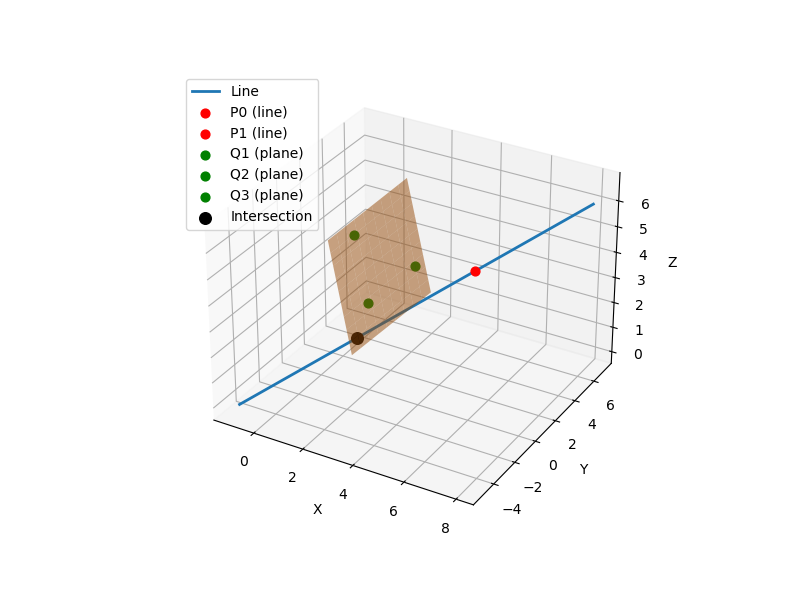
\includegraphics[width=0.5\columnwidth]{../figs/plot.png}
        \caption{Plot of given plane and line}
        \label{fig:fig}
    \end{figure}
\end{frame}
\end{document}
